%!TEX root=paper.tex
  
\newpage
\section{Overhead of the \tool}
\label{sec:overhead}

To measure the performance overhead of the \tool, we have implemented an automated benchmarking system. It is open source and available online and can be tested by the reader. \va{@Mircea: Don't forget to add link} The benchmark downloads the latest version of the \zee API and installs it in a Docker container. Then it calls several selected endpoints for 500 times each, tracking the response times. The endpoints are called in three different configurations: 

	\begin{enumerate}
		\item With no dashboard installed.
		\item With the dashboard enabled but with the outlier detection deactivated.
		\item With the dashboard enabled and the outlier threshold set to zero, thus effectively treating every request {\em like it were an outlier}.\footnote{This forces all the requests to be treated as outliers, and thus provides insight into this situation, which otherwise would be hard to generate}.
	\end{enumerate}

The last configuration is meant to evaluate the effect of the outlier detection as discussed in Section~\ref{sec:outliers} to the overall performance.
%
\Fref{fig:bench} and Table \ref{tab:benchmark} use violin plots and descriptive statistics, respectively, to present the distribution of response times resulting from running the benchmark for three different API endpoints on a quad-core machine, with Intel Core i5-4590 processor @3.30GHz, 8G of RAM and 240GB SSD disk drive.


\begin{figure}[h!]
	\centering
	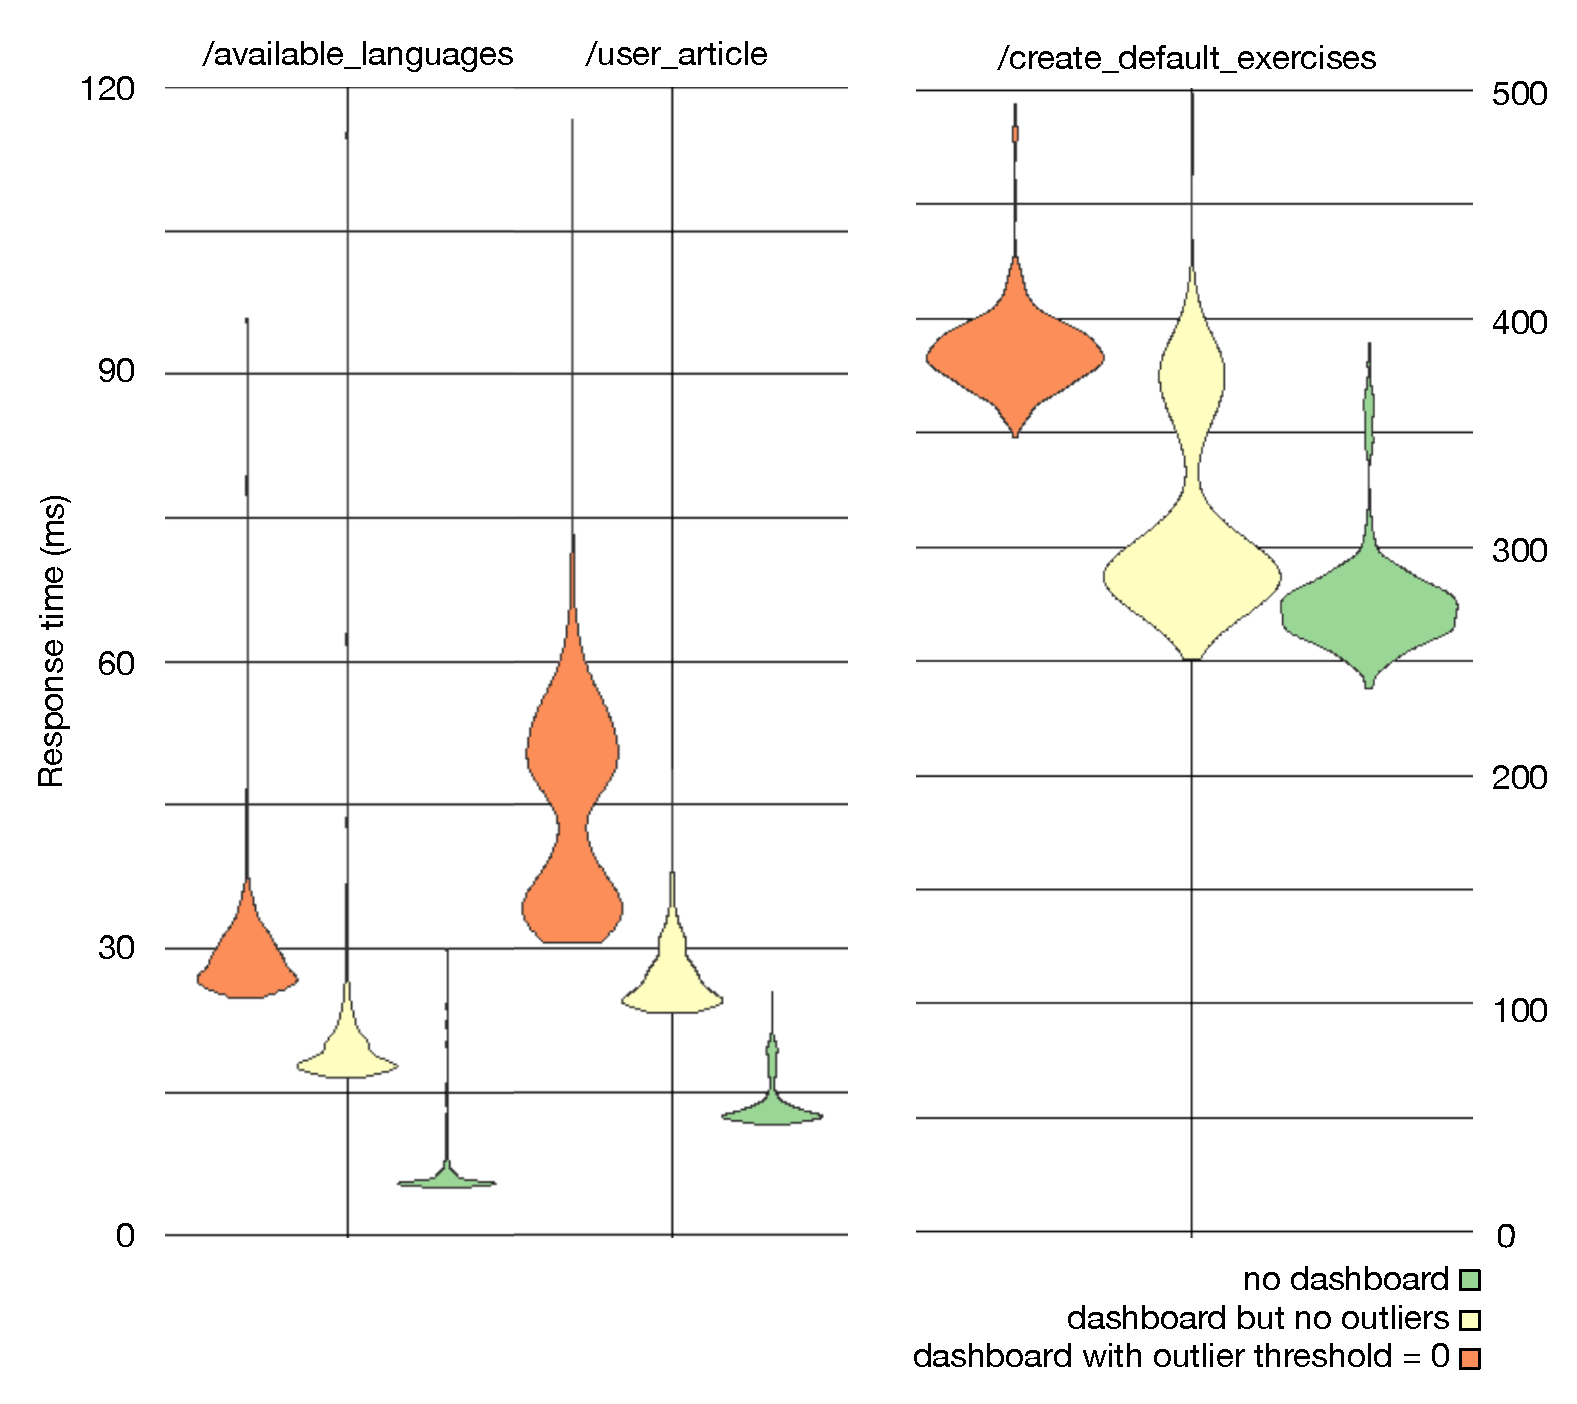
\includegraphics[width=\linewidth]{benchmark2.pdf}
	\caption{The distribution of response times when calling the three endpoints for 500 times in three conditions: no dashboard, dashboard but no outliers, dashboard and every request treated as an outlier}
	\label{fig:bench}
\end{figure}


%!TEX root=paper.tex

\newcommand{\yes}{\checkmark}

\begin{table}[tb]
	
	\centering

	\begin{tabular}{rllrr}
		\toprule
		\bfseries Endpoint & \bfseries Dash. & \bfseries All Out. & \bfseries Mean (ms) & \bfseries SD (ms) \\

		\midrule

	         available\_languages  &    &	    &   6.3 &  2.3 \\ 
	         available\_languages  &  \yes &    &  19.9 &  5.6 \\ 
	         available\_languages  &  \yes &  \yes &  29.4 &  5.4 \\ \\ 

	                user\_article  &    &	    &  13.9 &  2.6 \\
	                user\_article  &  \yes &    &  26.9 &  3.2 \\
	                user\_article  &  \yes &  \yes &  44.8 & 10.0 \\ \\

	    create\_default\_ex...     &    &	    &  276.0 & 22.4 \\ 
	    create\_default\_ex...     &  \yes &    & 313.6 & 43.2 \\
	    create\_default\_ex...     &  \yes &  \yes & 385.3 & 16.9 \\
	
		\bottomrule

	\end{tabular}
	\caption{Response times for three endpoints run 500 times in three different conditions each. Dash. = with dashboard. All Out. = every call being considered an outlier}
	\label{tab:benchmark}

\end{table}




	The three endpoints that are tested fall in two categories of complexity: 
	\begin{itemize}
		\item The two fast ones are very simple. 
		The first returns a list of language codes which are defined in the code, so it does not touch the \zee database. The second does a simple read from the database. 
		\item The slower endpoint does several complex writes to the database, so this is why it is much slower. However, in our case study, about half of the measured endpoints were at least as slow as this one, so its response time is representative.
	\end{itemize}

	The data shows that the dashboard (without outliers) introduces for the faster endpoints an overhead of~14ms and for the slower endpoint an overhead of~40ms, on average. 
	In the case of an outlier, the overhead is doubled, so the design decision of only collecting the extra information only for outliers seems to be validated. 
	Depending on the monitored application these numbers might be acceptable or not. In the case of the \zee case study, the maintainers find this overhead acceptable since they do not affect the overall user experience in any significant manner. 



  